%-------------------------------------------------------------------------------
\FloatBarrier\section{Human Capital}
%-------------------------------------------------------------------------------
The following graphs show the heatmap for the quartiles of selected skill measures and hourly local wages at age 35.

%-------------------------------------------------------------------------------
\FloatBarrier\subsection{Basics}
%-------------------------------------------------------------------------------
\begin{figure}[htp]\centering
\caption{Wages and AFQT scores}
\scalebox{0.35}{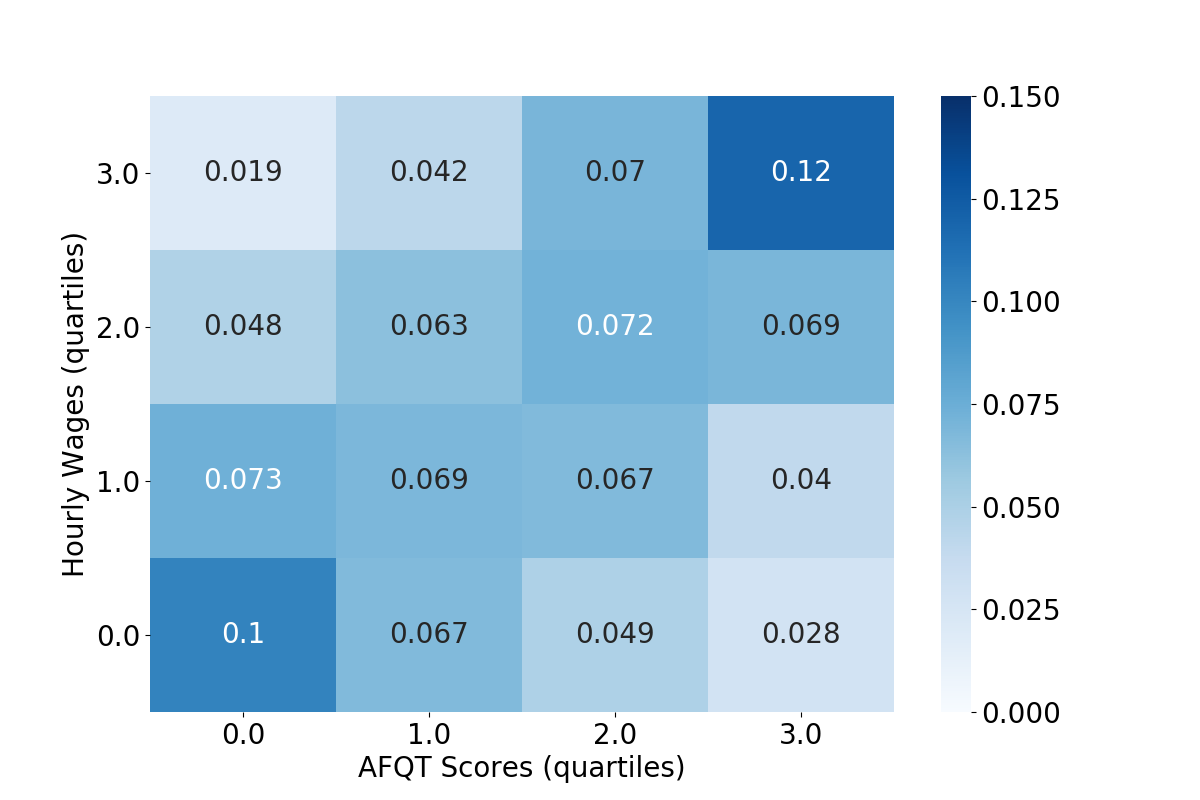
\includegraphics{fig-human-capital-basic-afqt}}
\end{figure}

\begin{figure}[htp]\centering
\caption{Wages and Rosenberg scores}
\scalebox{0.35}{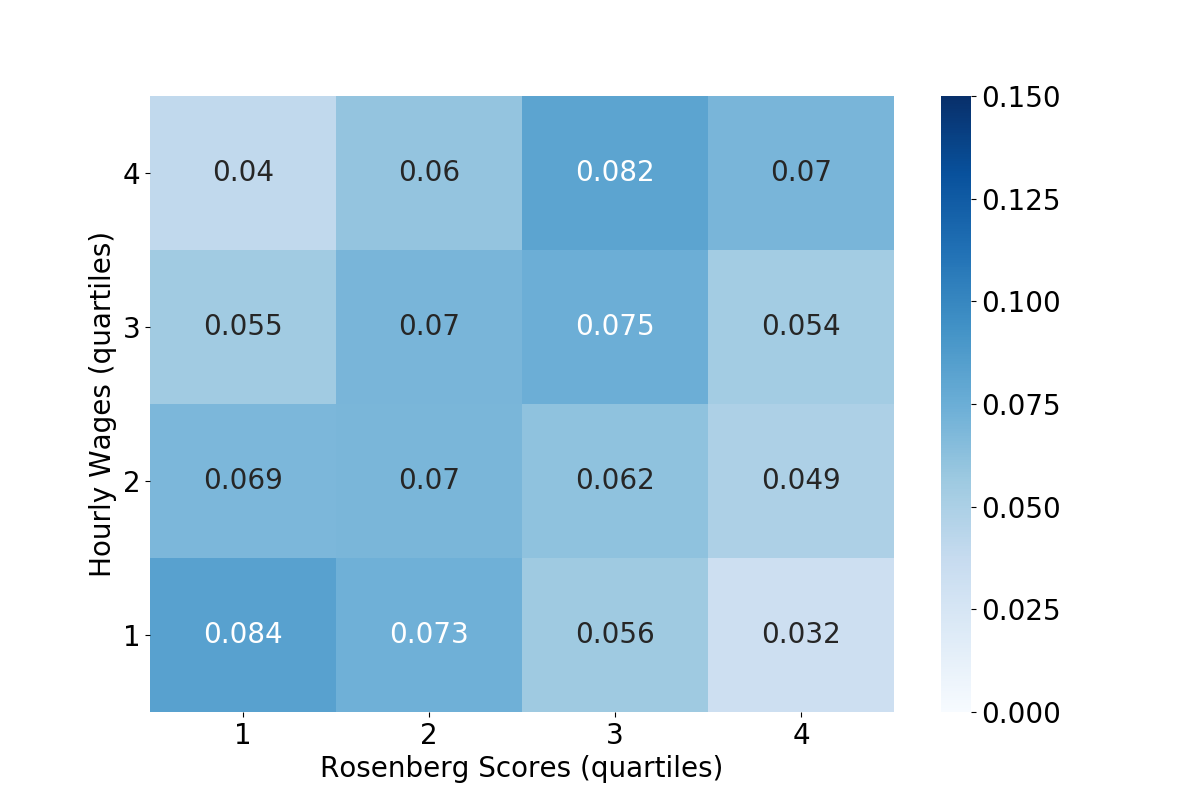
\includegraphics{fig-human-capital-basic-rosenberg}}
\end{figure}

\begin{figure}[htp]\centering
\caption{Wages and Rotter scores}
\scalebox{0.35}{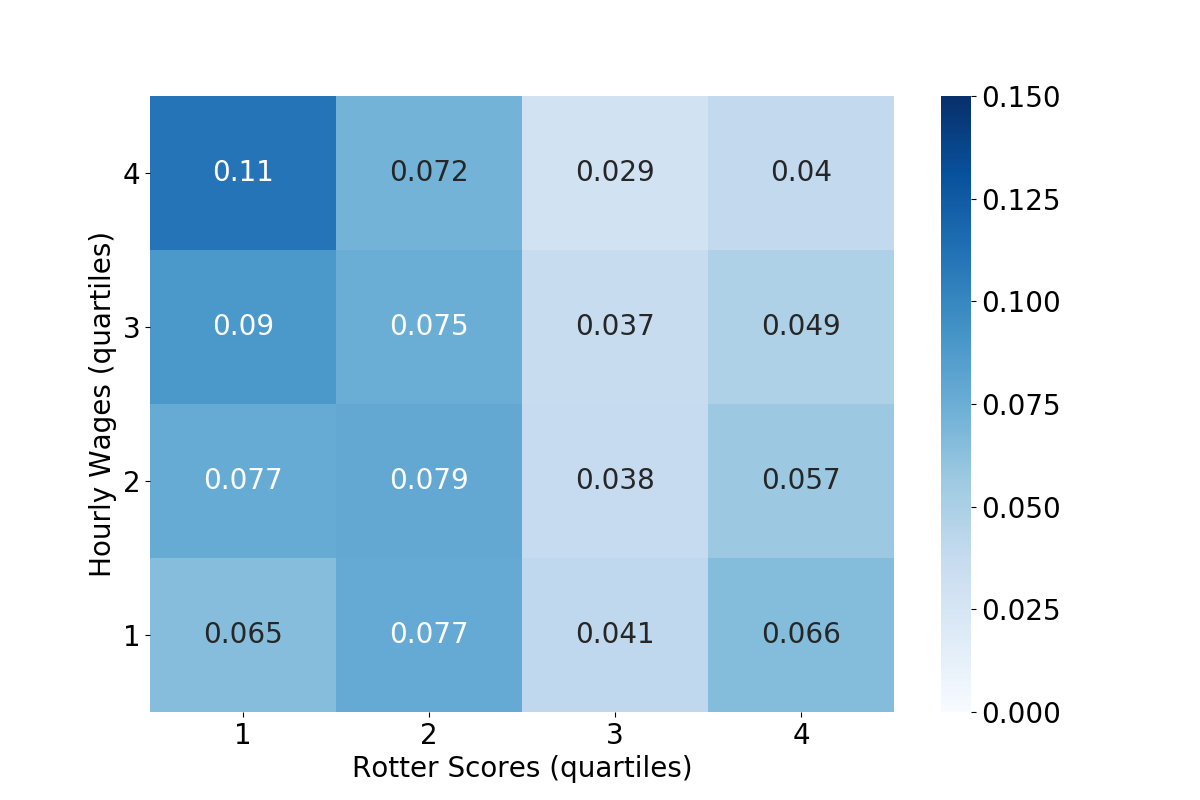
\includegraphics{fig-human-capital-basic-rotter}}
\end{figure}
%-------------------------------------------------------------------------------
\FloatBarrier\subsection{Differences by income quartile}
%-------------------------------------------------------------------------------
\begin{figure}[htp]\centering
\caption{Income quartile and AFQT scores}
\scalebox{0.35}{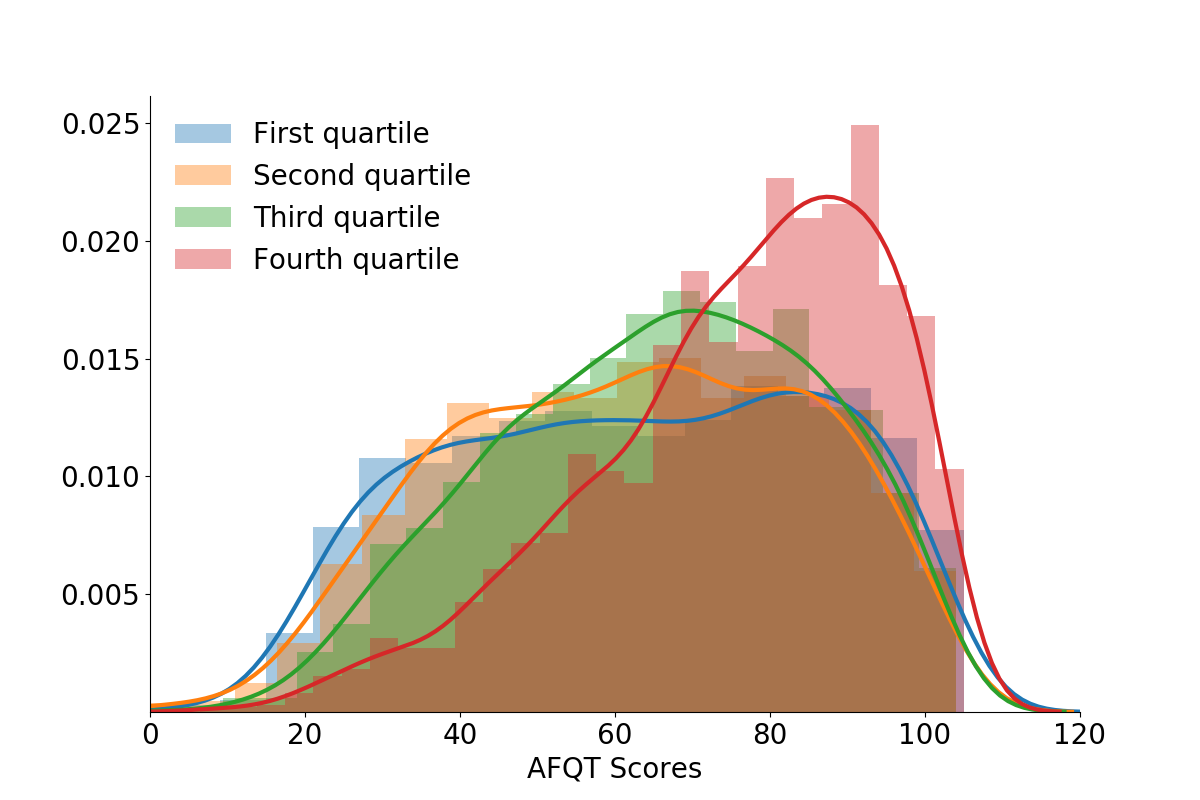
\includegraphics{fig-human-capital-income-quartile-afqt}}
\end{figure}

\begin{figure}[htp]\centering
\caption{Income quartile and Rosenberg scores}
\scalebox{0.35}{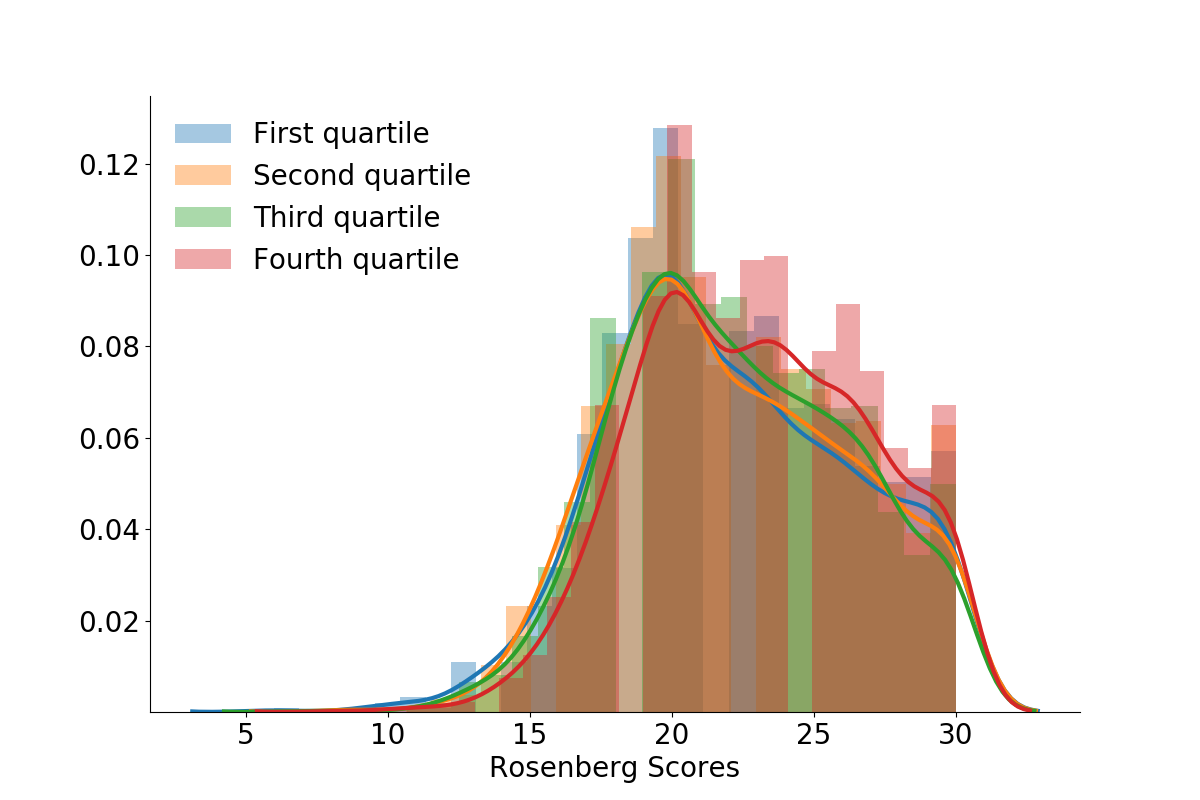
\includegraphics{fig-human-capital-income-quartile-rosenberg}}
\end{figure}

\begin{figure}[htp]\centering
\caption{Income quartile and Rotter scores}
\scalebox{0.35}{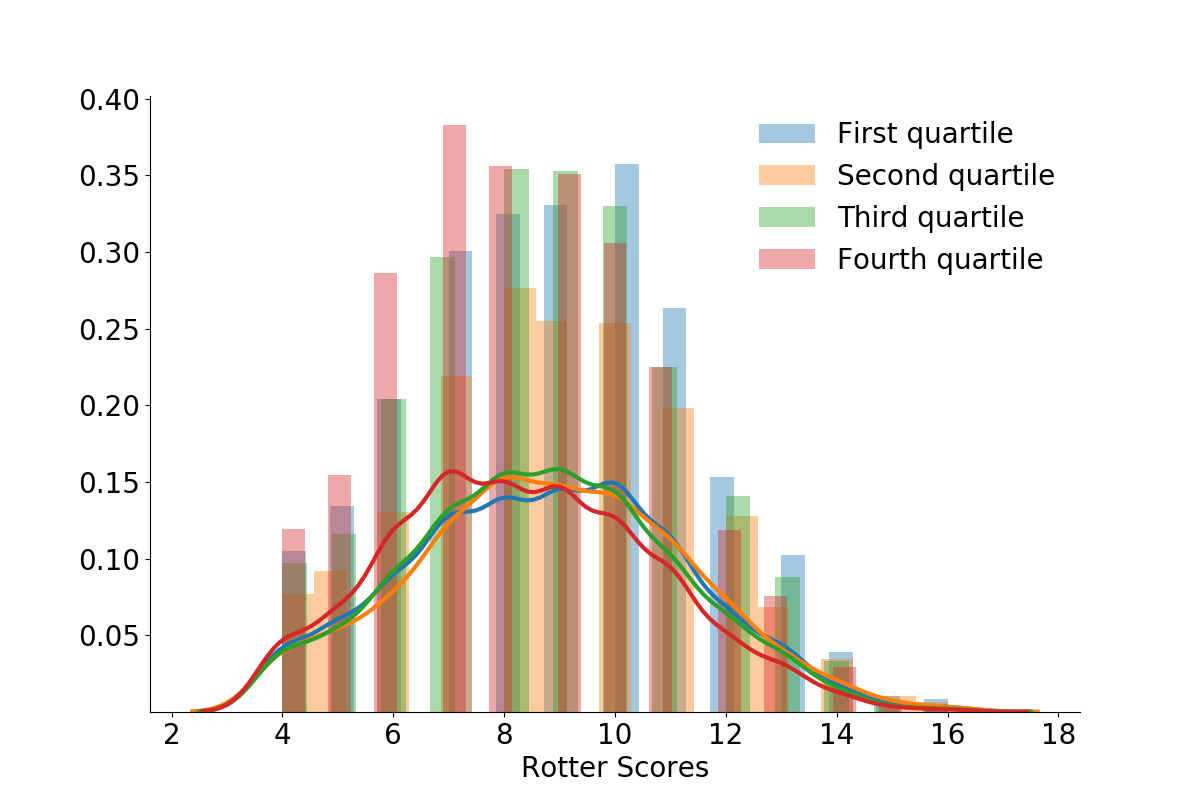
\includegraphics{fig-human-capital-income-quartile-rotter}}
\end{figure}
%-------------------------------------------------------------------------------
\FloatBarrier\subsection{Intergenerational Transmission}
%-------------------------------------------------------------------------------
\begin{figure}[htp]\centering
\caption{Mother's education and intergenerational transmission}
\scalebox{0.35}{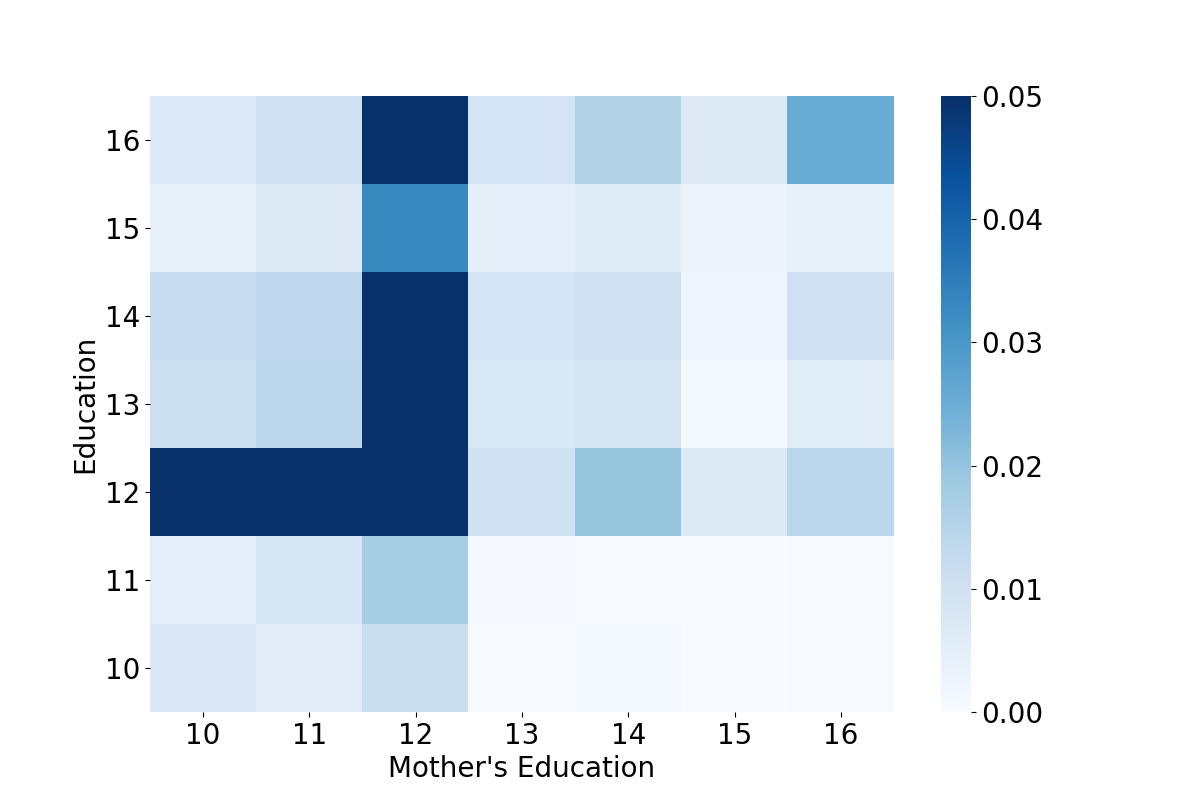
\includegraphics{fig-human-capital-intergenerational-mother}}
\end{figure}

\begin{figure}[htp]\centering
\caption{Father's education and intergenerational transmission}
\scalebox{0.35}{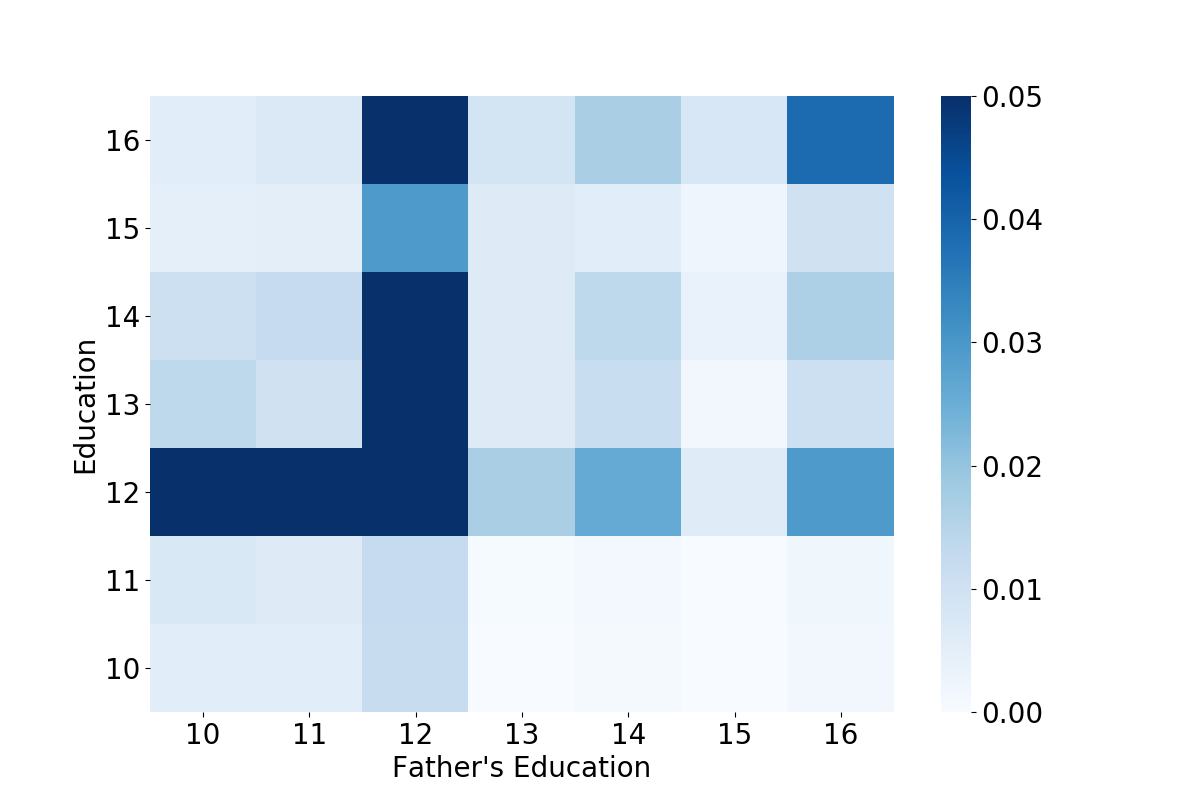
\includegraphics{fig-human-capital-intergenerational-father}}
\end{figure}


\begin{itemize}
\item On a high level there is a large literature on the distinction between nature and nurture.
\item Early childhood intervention programs are featured prominently in the discussion of policy responses.
\item The intergeneration transmission of human capital is gaining in strength, for example higher education is very costly in the United States. 
\end{itemize}
